\documentclass[conference]{IEEEtran}
\IEEEoverridecommandlockouts
% The preceding line is only needed to identify funding in the first footnote. If that is unneeded, please comment it out.
\usepackage{cite}
\usepackage{amsmath,amssymb,amsfonts}
\usepackage{algorithmic}
\usepackage{textcomp}
% \usepackage{latex-dev}
\usepackage{theorem,caption,extarrows,mathrsfs,physics,bm}
\usepackage{graphicx,xcolor,booktabs,subfigure}
\usepackage{tikz}
\usepackage[european]{circuitikz}
\usetikzlibrary{calc}
\usepackage{pgfplots,grffile}
\usepackage{fontspec}
\usepackage[skins]{tcolorbox}
\setmainfont{CMU Serif}
\setsansfont{CMU Sans Serif}
\setmonofont{Sarasa Fixed SC Nerd Font}
\pgfplotsset{compat=newest}
%% the following commands are needed for some matlab2tikz features
\usetikzlibrary{plotmarks}
\usetikzlibrary{arrows.meta}
\usetikzlibrary{calc}
\usepgfplotslibrary{patchplots}
\def\BibTeX{{\rm B\kern-.05em{\sc i\kern-.025em b}\kern-.08em
T\kern-.1667em\lower.7ex\hbox{E}\kern-.125emX}}
%% Define the theorem and proof
\newtheorem{theorem}[subsection]{Theorem}
\newtheorem{definition}[subsection]{Definition}
\newenvironment{thmbox}{\par
\vspace{4pt}
\begin{center}
	\tcbset{enhanced,notitle,colframe=black,colback=white}
	\begin{tcolorbox}[fuzzy shadow={1.6mm}{-1.6mm}{0mm}{0mm}{fill=black!90!white},arc=0mm]}{\end{tcolorbox}
\end{center}}
\usepackage{listings}
\lstset{
    basicstyle          =   \sffamily,          % 基本代码风格
    keywordstyle        =   \bfseries,          % 关键字风格
    commentstyle        =   \rmfamily\itshape,  % 注释的风格,斜体
    stringstyle         =   \ttfamily,  % 字符串风格
    flexiblecolumns,                % 别问为什么,加上这个
    numbers             =   left,   % 行号的位置在左边
    showspaces          =   false,  % 是否显示空格,显示了有点乱,所以不现实了
    numberstyle         =   \tiny\ttfamily,    % 行号的样式,小五号,tt等宽字体
    showstringspaces    =   false,
    captionpos          =   t,      % 这段代码的名字所呈现的位置,t指的是top上面
    frame               =   shadowbox,   % 显示边框
    rulesepcolor=\color{red!20!green!20!blue!20}
}

\lstdefinestyle{Python}{
    language        =   Python, % 语言选Python
    backgroundcolor=\color{backpycol},
    basicstyle      =   \ttfamily,
    numberstyle     =   \ttfamily,
    keywordstyle    =   \color{blue},
    keywordstyle    =   [2] \color{teal},
    stringstyle     =   \color{magenta},
    commentstyle    =   \color[HTML]{338AAF}\ttfamily,
    breaklines      =   true,   % 自动换行,建议不要写太长的行
    columns         =   fixed,  % 如果不加这一句,字间距就不固定,很丑,必须加
    basewidth       =   0.5em,
}
\definecolor{codegreen}{rgb}{0,0.6,0}
\definecolor{codegray}{rgb}{0.5,0.5,0.5}
\definecolor{codepurple}{rgb}{0.58,0,0.82}
\definecolor{backcolour}{rgb}{0.95,0.95,0.92}
\definecolor{backpycol}{rgb}{0.97,0.95,0.97}
\lstdefinestyle{C++}{
    language =[ANSI]C,
    backgroundcolor=\color{backcolour},
    commentstyle=\color[HTML]{338AAF}\ttfamily,
    keywordstyle=\sffamily\bfseries\color{magenta},
    numberstyle=\color{codegray},
    stringstyle=\color{codepurple},
    basicstyle=\ttfamily,
    breakatwhitespace=false,
    breaklines=true,
    basewidth=0.5em,
    captionpos=b,
    columns=fixed,
    frame=shadowbox,
    keepspaces=true,
    numbers=left,
    numbersep=5pt,
    showspaces=false,
    showstringspaces=false,
    showtabs=false,
    tabsize=4
}
\lstdefinestyle{matlab}{
    language=matlab,
    backgroundcolor=\color{backcolour},
    commentstyle=\color[HTML]{338AAF}\ttfamily,
    keywordstyle=\sffamily\bfseries\color{magenta},
    numberstyle=\color{codegray},
    stringstyle=\color{codepurple},
    basicstyle=\ttfamily,
    breakatwhitespace=false,
    breaklines=true,
    basewidth=0.5em,
    captionpos=b,
    columns=fixed,
    keepspaces=true,
    numbers=left,
    numbersep=5pt,
    showspaces=false,
    showstringspaces=false,
    showtabs=false,
    tabsize=4,
    frame=shadowbox
}
\definecolor{mygreen}{rgb}{0,0.6,0}
\definecolor{mygray}{rgb}{0.5,0.5,0.5}
\definecolor{mymauve}{rgb}{0.58,0,0.82}
\definecolor{bggray}{rgb}{0.93,0.95,0.94}
\lstdefinestyle{pseudocode}{
    backgroundcolor=\color{bggray},
    columns=fullflexible,
    tabsize=4,
    breaklines=true,               % automatic line breaking only at whitespace
    captionpos=b,                  % sets the caption-position to bottom
    commentstyle=\color{mygreen},  % comment style
    escapeinside={\%*}{*)},        % if you want to add LaTeX within your code
    keywordstyle=\color{blue},     % keyword style
    stringstyle=\color{mymauve}\ttfamily,  % string literal style
    frame=shadowbox,
    rulesepcolor=\color{red!20!green!20!blue!20},
    % identifierstyle=\color{red},
    language=c++,
    numbers=left,
    numberstyle=\small\color{codegray},
    basicstyle=\ttfamily,% size of fonts used for the code
    escapeinside=``,
    xleftmargin=0.6em,
    xrightmargin=0.6em,
    aboveskip=1em
}
\lstdefinestyle{Fortran}{
    language =fortran,
    backgroundcolor=\color{backcolour},
    commentstyle=\color[HTML]{338AAF}\ttfamily,
    keywordstyle=\sffamily\bfseries\color{magenta},
    numberstyle=\small\color{codegray},
    stringstyle=\color{codepurple},
    basicstyle=\ttfamily,
    breakatwhitespace=false,
    breaklines=true,
    basewidth=0.5em,
    captionpos=b,
    columns=fixed,
    frame=shadowbox,
    keepspaces=true,
    numbers=left,
    numbersep=5pt,
    showspaces=false,
    showstringspaces=false,
    showtabs=false,
    tabsize=4
}

\title{EE332 Lab2: Simulation of Full Adder on Nexys 4 DDR}
\author{
	\IEEEauthorblockN{1\textsuperscript{st} Qiu Kunyuan}
	\IEEEauthorblockA{
		\textit{EEE. Southern University of Science and Technology}\\
		Shenzhen, PRC\\
		11913019@mail.sustech.edu.cn
	}
}
\begin{document}
\maketitle
% !TEX root=./index.tex

\begin{abstract}
	This report focuses on the phenomenons encountered in the simulation of a simple full adder, to reveal some critical features of FPGA programming comparing to ordinary programmable devices. Among these phenomenons, jitters and the race-hazard conditions are of the most concerns.
\end{abstract}
\vspace{1em}
\begin{IEEEkeywords}
	FPGA, programmable logic, full adder, race-hazard condition, jitter, delay
\end{IEEEkeywords}

\section{Introduction}

Half adder and full adder are basic elements in digital circuits used to perform addition operations on binary numbers.

A \textit{half adder}

\begin{figure}[htpb]
	\begin{center}
		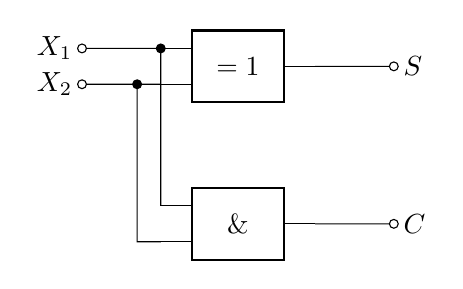
\begin{tikzpicture}
			\ctikzset{logic ports=european,tripoles/european not symbol=ieee circle}
			\draw
			(0,0) node[xor port] (xor1) {}
			(0,-2) node[and port] (and1) {}
			(xor1.out) to[short , -o] ++(1,0) node[right]{\(S\)}
			(and1.out) to[short , -o] ++(1,0) node[right]{\(C\)}
			(xor1.in 1) to[short, -o] ++(-1,0) coordinate(x1) node[left]{\(X_1\)}
			(xor1.in 1) to[short, *-] (and1.in 1)
			(xor1.in 2) -- ++(-0.3,0) coordinate(j1)
			(j1) to[short, *-] (j1 |- and1.in 2) -- (and1.in 2)
			(j1) to[short, -o] (x1 |- xor1.in 2) node[left]{\(X_2\)}
			;
		\end{tikzpicture}
		\caption{Gate Level Description of Half Adder}
		\label{HA_GateLevel}
	\end{center}
\end{figure}

is a combinational logic circuit shown in Figure.(\ref{HA_GateLevel}) that takes two binary inputs and produces two binary outputs: sum and carry.

\begin{eqnarray}
	\mathop{\mathrm{HA}}:(x_1,x_2)\mapsto(Q,C) :=
	\begin{cases}
		Q & =\mathop{\mathrm{xor}}(x_1,x_2) \\
		C & =\mathop{\mathrm{and}}(x_1,x_2)
	\end{cases}
\end{eqnarray}

The main limitation of the half adder is that it cannot handle carry inputs and therefore can only be used for 1-bit addition.

A \textit{full adder} is an extension of the half adder that accepts three binary inputs: two additions and a rounding input, and produces two binary outputs: sum and carry. Full adders can be connected in series to achieve binary addition of any number of bits.

\begin{figure}[htpb]
	\begin{center}
		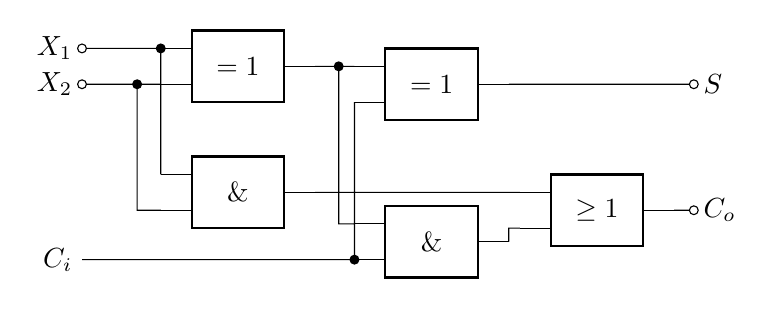
\begin{tikzpicture}
			\ctikzset{logic ports=european,tripoles/european not symbol=ieee circle}
			\draw
			(0,0) node[xor port] (xor1) {}
			(0,-1.6) node[and port] (and1) {}
			(xor1.out) ++(0.5,0) node[xor port, anchor=in 1] (xor2) {}
			(xor1.out) ++(0.5,-2) node[and port, anchor=in 1] (and2) {}
			(and1.out) ++(2.6,0) node[or port, anchor=in 1] (or1) {}
			(xor1.in 1) to[short, -o] ++(-1,0) coordinate(x1) node[left]{\(X_1\)}
			(xor1.in 1) to[short, *-] (and1.in 1)
			(xor1.in 2) -- ++(-0.3,0) coordinate(j1)
			(j1) to[short, *-] (j1 |- and1.in 2) -- (and1.in 2)
			(j1) to[short, -o] (x1 |- xor1.in 2) node[left]{\(X_2\)}
			(x1 |- and2.in 2) coordinate(ci) node[left]{\(C_i\)}
			(xor1.out) -- ++(0.3,0) coordinate(j2) to[short, *-] (xor2.in 1)
			(j2) |- (and2.in 1)
			(ci) -| (and2.in 2)
			(and2.in 2) to[short, *-] (xor2.in 2)
			(and1.out) |- (or1.in 1)
			(and2.out) |- (or1.in 2)
			(or1.out) to[short, -o] ++(0.25,0) coordinate(co) node[right]{\(C_o\)}
			(xor2.out) to[short, -o] (co |- xor2.out) node[right]{\(S\)}
			;
		\end{tikzpicture}
		\caption{Gate Level Description of Full Adder}
		\label{FA_GateLevel}
	\end{center}
\end{figure}

Implementation of full adder can be derived directly from 3-digit addition, where the final carry output is toggled if any of \(X_1+X_2\) or \(C_i+Q_1\) produces a carry:

\begin{eqnarray}
	(q_1,c_1)&=\mathop{\mathrm{HA}}(x_1,x_2) \\
	(q_2,c_2)&=\mathop{\mathrm{HA}}(q_1,c_i) \\
	c_o &= \mathop{\mathrm{or}}(c_1,c_2)
\end{eqnarray}

Therefore the gate-level circuit of the full adder can be easily captured, as shown of Figure.(\ref{FA_GateLevel})

\section{Verilog Modeling}

There are two levels of HDL modeling for full adder, one for gate level description and one for behavioral level description.

\subsection{Gate-Level Implementation}

\lstinputlisting[caption={Gate Level Modeling of Full Adder in Verilog}, language=verilog, style=verilog, label=glm_fa, linewidth=0.92\linewidth]{../../lab2/lab2.srcs/sources_1/new/full_adder_g.v}

For the gate level modeling, the DNF (OR-AND) of the output ports are required:

\begin{eqnarray}
	\begin{aligned}
		Q_2              & =HA(HA(x_1,x_2)[0],c_i)[0]                                           \\
		                 & =\mathop{\mathrm{xor}}(\mathop{\mathrm{xor}}(x_1,x_2),c_i)           \\
		                 & = \overline{AB} C+\overline{A} B \overline{C} + A \overline{BC} +ABC \\
		C_{\mathrm{out}} & =AB+BC+AC
	\end{aligned}
\end{eqnarray}

Therefore, the Verilog code is pretty straight forward, as the Code.(\ref{glm_fa}). For the Vivado elaboration and synthesis process, the logic functions are expanded to its DNF, meaning only AND/OR/NOT gates remains in the elaborated schematic:

\begin{figure}[htpb]
	\begin{center}
		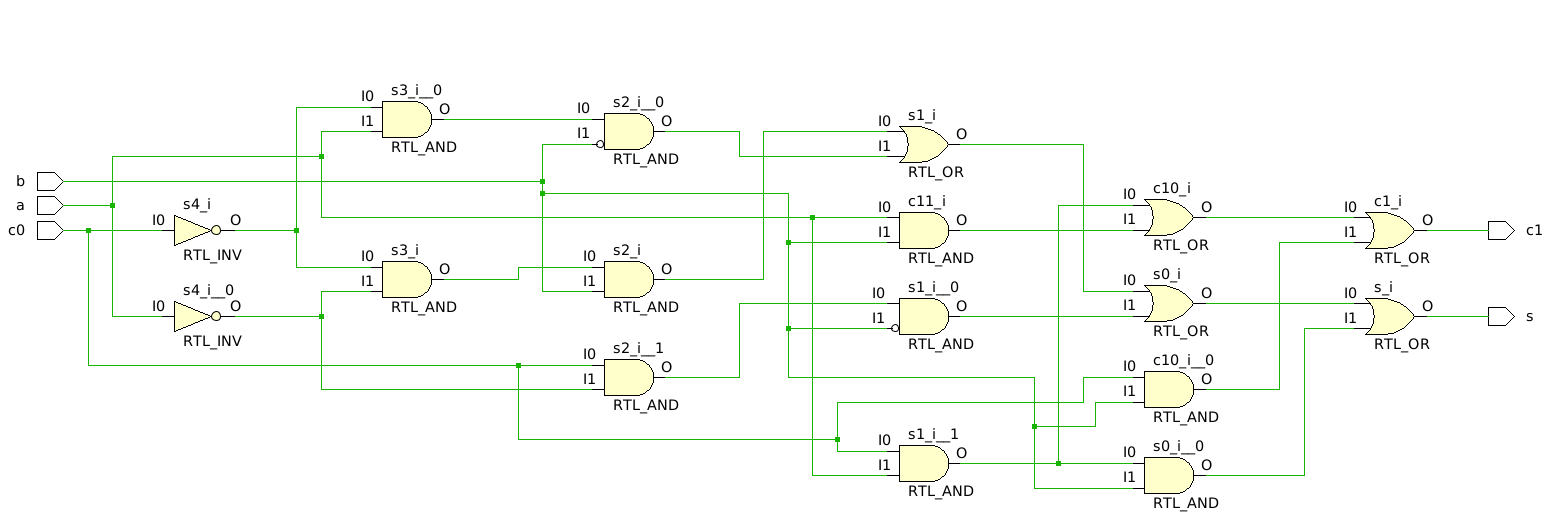
\includegraphics[width=0.97\linewidth]{report_lab2.assets/20240307171752.png}
		\caption{Elaborated Gate Level Description}
		\label{elaborated_gl_sch}
	\end{center}
\end{figure}

\subsection{LUT Implementation}

\lstinputlisting[caption={Gate Level Modeling of Full Adder in Verilog}, language=verilog, style=verilog, label=glm_fa, linewidth=0.92\linewidth]{../../lab2/lab2.srcs/sources_1/new/full_adder_lut.v}

The combine logic functions are implemented by LUT(Look-Up Table)s inside the FPGA components in real world, while the half adder is a common LUT element inside the CLBs. By simply configuring the switchable connections between the CLBs and the controlling MUXs inside the CLBs, a cascaded design can be easily obtained.

\begin{figure}[htpb]
	\begin{center}
		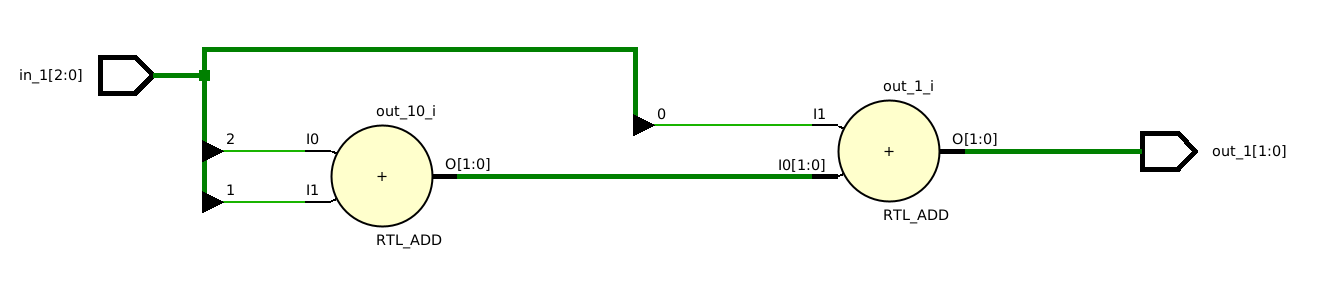
\includegraphics[width=0.97\linewidth]{report_lab2.assets/20240307172354.png}
		\caption{Elaborated RTL Level Description}
		\label{elaborated_lut_level_sch}
	\end{center}
\end{figure}

\subsection{Synthesized Implementation}

\begin{figure}[htpb]
	\begin{center}
		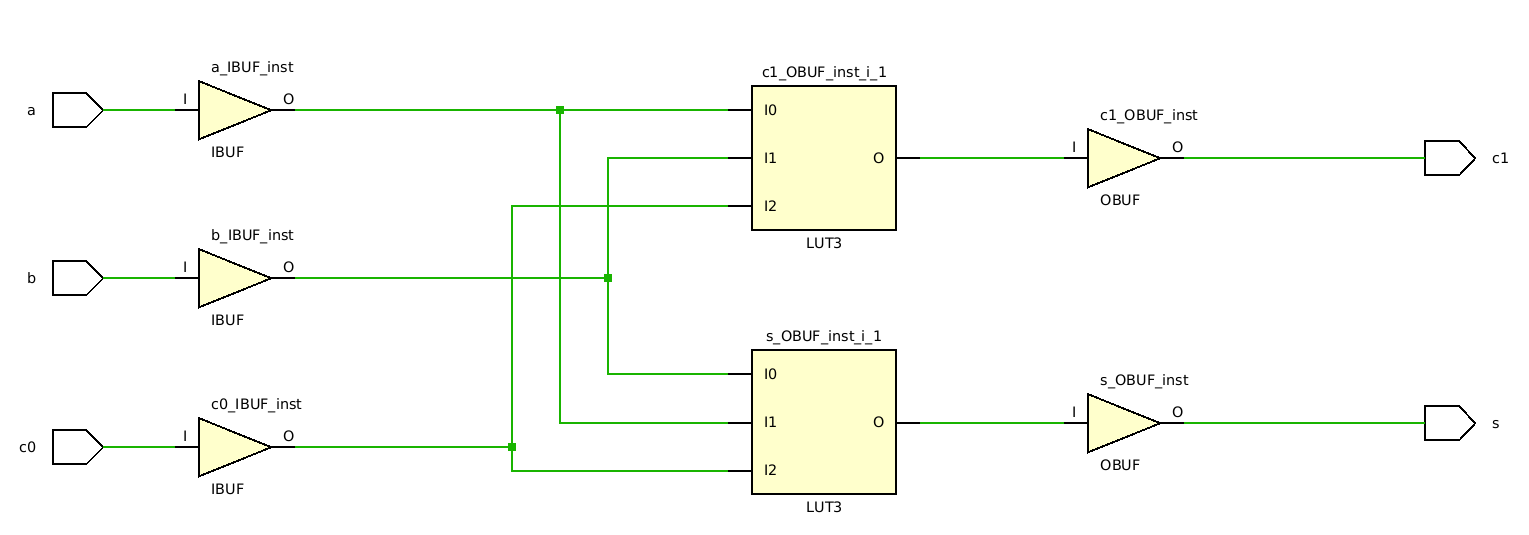
\includegraphics[width=0.97\linewidth]{report_lab2.assets/20240307172835.png}
		\caption{Synthesized Design}
		\label{FA_synth}
	\end{center}
\end{figure}

Either the gate level design (\ref{elaborated_gl_sch}) or the RTL level design (\ref{elaborated_lut_level_sch}) are synthesized into the same schematic (\ref{FA_synth}) after the synthesis and implementation process, since the FPGA device only provide configurable LUT as the measure to combinational logic inside the CLB.

In the synthesized schematic (\ref{FA_synth}), the two LUT cells are combinational logic functions of \(S=\mathop{\mathrm{LUT_1}}(X_0,X_1,C_i)\) and \(C_o=\mathop{\mathrm{LUT_2}}(X_0,X_1,C_i)\) respectively.

\section{Simulation}

\begin{table}
	\begin{center}
		\begin{tabular}[htb]{ccccccc}
			\toprule
			\(X_1\) & \(X_0\) & \(C_i\) & \(\mathop{\mathrm{dec}}(in[2:0])\) & \(C_o\) & \(S\) & \(\mathop{\mathrm{dec}}(out[1:0])\) \\
			\midrule
			0       & 0       & 0       & 0                                  & 0       & 0     & 0                                   \\
			0       & 0       & 1       & 1                                  & 0       & 1     & 1                                   \\
			0       & 1       & 0       & 2                                  & 0       & 1     & 1                                   \\
			0       & 1       & 1       & 3                                  & 1       & 0     & 2                                   \\
			1       & 0       & 0       & 4                                  & 0       & 1     & 1                                   \\
			1       & 0       & 1       & 5                                  & 1       & 0     & 2                                   \\
			1       & 1       & 0       & 6                                  & 1       & 0     & 2                                   \\
			1       & 1       & 1       & 7                                  & 1       & 1     & 3                                   \\
			\bottomrule
		\end{tabular}
		\caption{Truth Table of Full Adder}
		\label{tt_fa}
	\end{center}
\end{table}

The truth table of the full adder is Table.(\ref{tt_fa}).

\end{document}